\section{Inverse Engineering Approach}
 It is clear from equation \eqref{eq:stacurvature} that the choice of $ u_{sta} $ is crucial to guarantee the stability of the protocol over a wide range of initial velocities and to ensure that the outcoming particle does not experience any kind of transverse excitation (as in \cref{fig:setup}) after the bent section.
 In particular, for a total travel time $ 2T $, the following constraints have been set:
 \begin{align}
 &	u_{sta}(0) =\dot{u}_{sta}(0) = \ddot{u}_{sta}(0) = 0 , \label{eq:boundary0}\\
 &	u_{sta}(T) = \Delta u_{sta}, \hspace{3em } \dot{u}_{sta}(T) = \ddot{u}_{sta}(T) = 0, \label{eq:boundary1}\\
 &	u_{sta}(2T) =\dot{u}_{sta}(0) = \ddot{u}_{sta}(0) = 0, \label{eq:boundary2}
 \end{align}
 where $ \Delta u_{sta} $ is the maximum transverse displacement in the middle of the curve and it is fixed by the physics of the system.
 A natural choice for $u_{sta}$ is a polynomial fulfilling the \crefrange{eq:boundary0}{eq:boundary2}.
 In \cite{QuantumControlImpens2020} the symmetry of the problem has been  exploited  by using $ u_{sta}(t)  = P(t/T)$ for the first section (i.e. for $ t \in [0,T]$) and the polynomial $ P(2-t/T) $ for $ t \in [T,2T] $ .
 Following the constraints of \crefrange{eq:boundary0}{eq:boundary2}, Gu{\'e}ry et al. choice for the polynomial is 
 \begin{equation}
	 \label{eq:order1poly}
 	P(\tau) = \Delta u_{sta}(10\tau^3 - 15\tau^4 + 6\tau^5) 
 \end{equation}
The resulting curvature presents a cusp in the centre of the path, due to the fact that the trajectory was defined on the half interval.
\begin{figure}
	\centering
		\begin{overpic}[scale = 1]{gfx/curves.pdf}
			\put(17,34){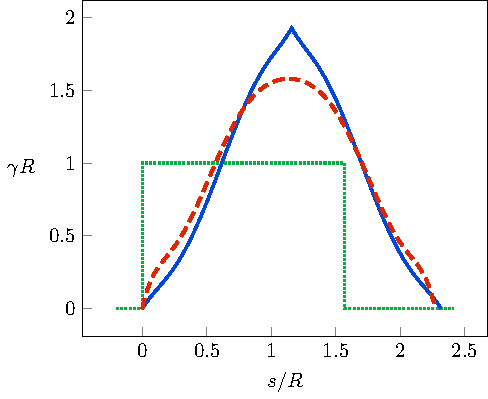
\includegraphics[scale = .55]{gfx/curvatures.pdf}}
		\end{overpic}
	\caption{View from the top of the curves for different $ n $. In this case $ k_{0}R = 500 $ and $ \omega T = 5 $. In the inset the comparison of different curvatures obtained by  setting different $ n $ is shown. We can see that for $ n \neq 1 $ the curvatures are smooth function witn cusps for $ t = T $ }
	\label{fig:curvatures}
\end{figure}
This may cause numerical instabilities and therefore we decided to use different trajectories defined on the whole interval $ [0,2T] $ and we will refer to them with the notation $U(t)$.
Moreover, we imposed the derivatives in \crefrange{eq:boundary0}{eq:boundary2} to be 0 up to the $ n^{th} $ order, so we can rewrite the boundary conditons are
\begin{align}
&	U^{(i)}(0) = 0 ~ \mathrm{for} ~  i = 0, ..., n, \\
&	U^{(0)}(T) = \Delta U, ~ U^{(i)(T)}=0 ~ \mathrm{for} ~ i = 1, ..., n, \\
&	U^{(i)}(2T) = 0 ~ \mathrm{for} ~ i = 0, ..., n.
\end{align}
We then tested the protocol for different $ n $ and we would like to remark that for each $n$ we evaluated the corresponding $ \Delta U_{n}  $ and $ T_{n} $.
In the remainder of the work we will identify every trajectory by the number $ n $ and to keep the notation consistent we will refer to $ u_{sta} $ as $ U_{1} $.
We will do the same for the curvature $ \gamma_{n} $ and the corresponding $ \Ga_{n} $. 
In \cref{fig:curvatures} we can see how the resulting curvatures are smoother functions and do not show any cusps in the middle.
Using the curvatures obtained applying the STA approach with different trajectories, we are now ready to simulate the evolution of the quantum state under the effects of the corresponding Hamiltonian.
